\section{Street Network Analysis}\label{network-analysis}

The intuition of networks (graphs) is that nodes (vertices) are connected by links (edges) to other nodes. For example, a social network may consist of individuals connected through relationships with one another. Network analysis can then be used to answer how connected or `relatively central' a particular person is, thus inferring their structural importance within the network. Two of the more common measures of importance are \emph{closeness centrality} \cite{Sabidussi1966}, how closely a node is located to other nodes, and \emph{betweenness centrality} \cite{Freeman1977}, how often a node provides the shortest path between other nodes. The computation of these measures involves the use of algorithms calculating \emph{shortest-paths} through the network: in the basic case, distance is topological: the number of nodes between origin and destination pairs. It is also possible to represent distance by assigning a traversal cost to the links between the nodes. For example, in street networks, these traversal costs can correspond to the lengths of streets (links) between road intersections (nodes).

To understand the contemporary context of street network analysis in practice --- and potential ramifications for closeness centrality --- it is beneficial to be aware of the literature and distinctions related to \emph{global} and \emph{localised} forms of analysis; differences in street network representation; the use of \emph{topological}, \emph{metric}, and \emph{geometric} distances as a heuristic for determining shortest paths through the network; and the impact of network topology on the robustness and comparability of results. For clarity and reproducibility, this section provides an overview of these distinctions and related background literature prior to introducing the technicalities of closeness centralities in the next section.

\subsection{Scales of Analysis}

Network centrality methods can be applied to the entirety of a network, e.g., for a given city, which is typically referred to as `global' analysis. In this case, the magnitude of the resultant network centrality is coupled to the size of the network with the implication that the larger the network, the larger the centrality values. Different boundary definitions therefore lead to fluctuating centrality values, raising some issues:
\begin{itemize}
  \item It is difficult to rigorously and consistently define boundaries from city to city. This problem is exacerbated for large urban agglomerations or when the boundaries between urban areas are not clearly delineated. One solution is to apply a technique such as network percolation \cite{Arcaute2016} to heuristically delineate boundaries;
  \item Global analysis is subject to significant ``edge-effects'', where centrality values diminish towards the edge of the network because the algorithms are constrained by the boundary. This may be manageable when using rigorous boundary definitions, but otherwise creates significant issues for comparability and generalisability \cite{Turner2007, van_nes_introduction_2021};
  \item More localised phenomena within networks cannot be directly analysed or compared because local-scale properties are masked by the global-scale characteristics of the network \cite{Porta2009, van_nes_introduction_2021}. This makes it difficult to meaningfully compare localised properties of networks between locations, particularly from the point of view of urban design and planning interventions where it is necessary to gauge local-scale impacts of design decisions.
\end{itemize}

These issues are mitigated through the use of ``localised'' network analysis which works by iteratively visiting each node using a windowing methodology to define a local catchment area for analysis \cite{Turner2007}. This intuition is conveyed in Figure~\ref{fig:moving_window}: each node is visited in turn, all other reachable nodes within a selected distance threshold are then identified and isolated from the network at large before the analysis then proceeds (using only the locally extracted sub-graph). The algorithm then steps to the next node and repeats the process until the entirety of the network has been visited.

\begin{figure}[htbp]
  \centering
  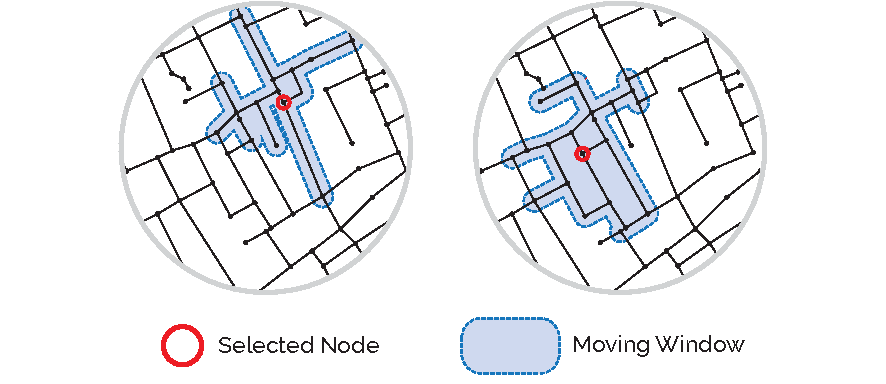
\includegraphics[width=\linewidth, keepaspectratio]{../images/moving_window.pdf}
  \caption{Moving window catchment area.}\label{fig:moving_window}
\end{figure}

Localised methods confer several advantages:
\begin{itemize}
  \item A measure computed for a given distance threshold on one network can be compared directly to the same measure and distance threshold computed for another location --- even in a different city --- because the localised boundary extents are defined in a methodologically consistent manner from location to location;
  \item Localised analysis substantially mitigates edge-effects as long as the network is adequately buffered relative to the considered distance threshold (for example, if using a 1km local catchment then a 1km buffer will eliminate edge effects);
  \item Centralities can be computed for a range of nearer or farther distance thresholds (commonly referred to as radii) to draw-out smaller or larger structures within the network. A number of different distance thresholds is ordinarily computed to understand the properties of the street network at different scales of analysis. Use of smaller distances can yield information about local-scale walkability whereas the use of larger distances can offer larger-scale insights equivalent to global methods without the aforementioned drawbacks such as edge effects.
\end{itemize}

The use of localised network analysis is therefore conventional in current practice; the remainder of this discussion and the ensuing analysis is based on the localised form of analysis. In common parlance, localised measures computed for larger radii (e.g. 10km or 20km) are sometimes sometimes termed as `global' analysis in the literature. To avoid terminological inconsistency, we refer to `localised' analysis regardless of the local distance threshold used.

\subsection{Model Representations}\label{network-representations}

The \emph{primal} representation is when intersections are represented by nodes and streets by links, thus corresponding to conceptions of streets embedded in euclidean space: intersections adopt specified coordinates connected by streets to other intersections \cite{Porta2006a}. \emph{Space Syntax}, on the other hand, emerged around the use of the \emph{dual} representation \cite{Hillier1984}. This originated with the use of \emph{axial lines} to generate a topological representation of urban space. An \emph{axial line} is an uninterrupted longest line of sight connecting convex spaces (an area where any two points can be connected by a straight line), potentially spanning multiple contiguous street segments, and distances are topological, meaning the number of steps from axial line to axial line. This is a form of \emph{dual} representation where the nodes represent street corridors and the links represent the topological steps between them. The techniques for the extrapolation of \emph{axial lines} from the street network can be complex and variable, historically leading to debates on whether it is possible to do so in an algorithmically rigorous manner \cite{Ratti2004, Turner2005a, Porta2006a}. It is important to recognise that newer and more tractable forms of dual representation have since been widely adopted by the space syntax community: \emph{fractional analysis} and the now prevalent \emph{angular segment analysis} \cite{Turner2000, Dalton2001, Turner2005a, Turner2007} forego axial lines, instead deriving the network from road centre-lines through a direct inversion of the \emph{primal} representation into its \emph{dual}, as shown in Figure~\ref{fig:primal_vs_dual}. Nodes therefore correspond to the mid-points of street segments and links typically correspond to the \emph{geometric distance} (angular change) linking them, though can also represent \emph{metric distance} (such as metres), as is typically the case for \emph{primal} representations \cite{Rosvall2005, Marshall2018, Batty2004}. Forms of distance are discussed in the following sub-section.

\begin{figure}[htbp]
  \centering
  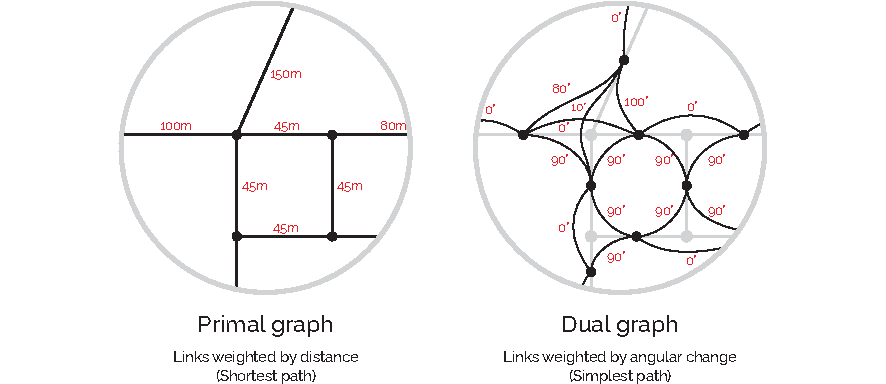
\includegraphics[width=\linewidth, keepaspectratio]{../images/primal_vs_dual.pdf}
  \caption{The \emph{primal} street network representation with \emph{metric distances} (left) and a corresponding example of a dual representation (right) with \emph{geometric distances}. Note that the dual network can be used with \emph{metric distances}.}\label{fig:primal_vs_dual}
\end{figure}

There is a large variety of potential network representations \cite{Marshall2018}, some of which can be used to analyse properties such as the connectivity of the network and its \emph{small-world} and \emph{scale-free} characteristics, emblematic of complex systems and network analysis more generally \cite{Albert2002, Porta2006a}. However, contemporary forms of street network analysis tend to adopt a pragmatic approach which leverages the widespread availability of street network datasets, typically used either directly in the \emph{primal} representation or its direct \emph{dual} inversion.

\subsection{Cost parameters}

Network links (edges) can be assigned a cost parameter to reflect distances incurred by traversing a particular link. Historically, \emph{topological distances} were used in the context of axial representations. Contemporary approaches more typically make use of \emph{metric distances} or \emph{geometric distances}. The former is ordinarily used with physical distance units such as metres whereas the latter approach is instead based on angular deviation, or in other terms the linearity of routes. Simpler routes with better lines-of-sight are therefore considered `shorter' than more convoluted routes even if the euclidean distances are greater; thus, routes requiring minimal geometric complexity are favoured to routes requiring minimal physical effort \cite{Hillier2007, Serra2019}. This tends to be the preferred distance metric in space syntax, where geometric properties of the street network are seen as important determinants in the general evolution of land-uses and the wider patterns of activities in cities \cite{Penn1998}.

The use of \emph{geometric distance} introduces an implementation nuance in that shortest-path algorithms will `bypass' sharp angular turns in cases where smaller combinations of adjacent angles can be combined instead (Figure~\ref{fig:enforced_dual}), thus making it necessary to enforce directional constraints for algorithms as they pass-through nodes during graph traversals \cite{Turner2007}. Note that unlike tailored network analysis tools such as \emph{depthmapX} \cite{turner_depthmapx_2020}, \emph{Place Syntax Tool} \cite{stahle_place_2023}, or \emph{cityseer}  \cite{simons_cityseer_2023}, generic network analysis packages typically do not take this into account and would also not necessarily return symmetrical routes if the direction of travel were reversed \cite{banino_vector-based_2018}.

\begin{figure}[htbp]
  \centering
  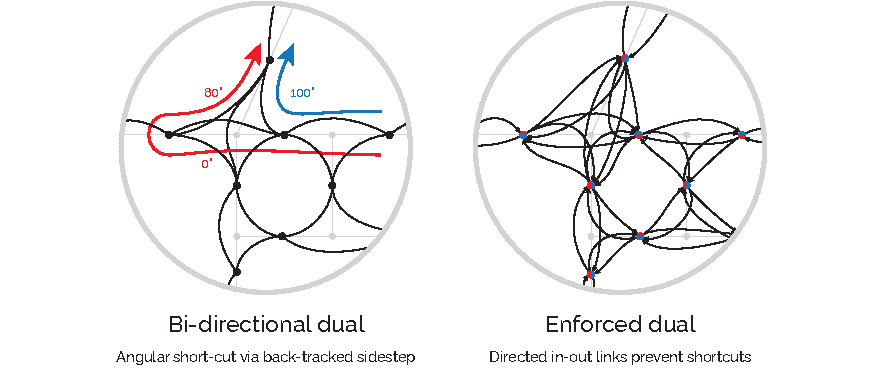
\includegraphics[width=\linewidth, keepaspectratio]{../images/enforced_dual.pdf}
  \caption{Shortest angular path side-stepping.}\label{fig:enforced_dual}
\end{figure}

\emph{Metric distance} and \emph{geometric distance} as a cost parameter are not mutually exclusive. While expressing distances differently, both are valid approaches and their interrelation is complex \cite{Barthelemy2015}. Pedestrian route choices may vary from place to place and from person to person. Shortest routes are frequently the same for either cost parameter \cite{Viana2013, Omer2018} and strong correlations are observed between them for certain distances \cite{Hillier2007, Serra2019}. Modal choice presents an additional nuance \cite{Serra2019}; research has shown strong support for \emph{geometric distances} within the context of vehicular travel, particularly at distances larger than 2000m. However, there are indications that \emph{metric distances} retain relevancy for smaller scale analysis and for non-vehicular forms of transport such as cycling \cite{Serra2019, sharmin_meta-analysis_2018}.

Note that \emph{metric distances} can be computed on the \emph{dual} and that \emph{geometric distances} can technically also be computed on the \emph{primal}, and that it is also possible to simultaneously apply multiple representations \cite{Masucci2016}.

\subsection{Distortions related to topology and geometry}

Network analysis algorithms are sensitive to the topological structure of the network, and low-quality network datasets will therefore lead to spurious results. For example, broken links will misroute shortest-path algorithms and unnecessarily complex representations of features such as intricate road intersections will introduce inflated centralities to the surrounding network.

A common problem is the conflation of the topological structure of the network with the geometrical trajectories of streets, which introduces different intensities of nodes for equivalent lengths of streets segments. For example, a straight street segment may be represented as a single link between two nodes whereas an arced street of equivalent length is often represented with additional nodes to approximate the geometric curvature of the roadway. Each additional node results in more summations when calculating centralities, consequently skewing the outcome of measures. It is therefore important to use cleaned network representations which maintain the distinction between the geometric representation of roadways and the topological structure of the network. If using more topologically complex networks from sources such as OpenStreetMap, then it is generally necessary to first clean and simplify the network. This should be done while preserving the geometry of the original street segments so that accurate distances or angular changes in direction can be measured \cite{gil_road_nodate}. In this research, these techniques are facilitated by the \texttt{cityseer-api} package \cite{simons_cityseer_2023}. There is wider interest within the network analysis community in the formalisation and standardisation of network simplification methods \cite{krenz_employing_nodate}.

Another manifestation of this phenomenon is the topological divergence between \emph{primal} and \emph{dual} representations (see Figure~\ref{fig:primal_vs_dual_structure}). Even though both derive from the same underlying structure, the outputs for the same network measures using the same cost parameters will yield different results; the \emph{dual} representation generates higher equivalent metrics due to larger quantities of nodes and links, which becomes more pronounced as the complexity of the network increases. Comparative evaluation between \emph{metric distance} measures on \emph{primal} networks and \emph{geometric distance} measures on \emph{dual} networks should be avoided because the outcomes will also reflect representational differences.

\begin{figure}[htbp]
  \centering
  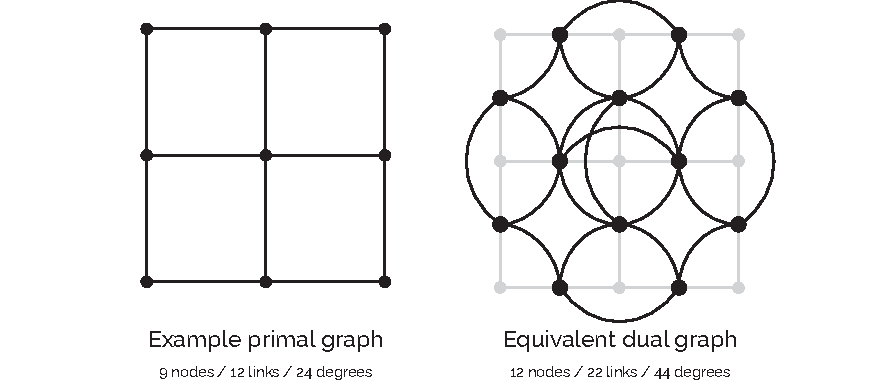
\includegraphics[width=\linewidth, keepaspectratio]{../images/primal_vs_dual_structure.pdf}
  \caption{Topological divergence of primal and dual representations.}\label{fig:primal_vs_dual_structure}
\end{figure}
